\chapter{Tabel Kemajuan Reaksi}\label{ch:g10:reaction-progress-table}

% ledger: use:NaN3-airbag
Dalam sebuah tabrakan mobil, sebuah bantalan menyembur keluar dari roda
kemudi dan terisi gas dalam sepersekian detik, sebelum kepala pengemudi
terlempar ke depan. Gas itu dihasilkan oleh sebuah \omterm{def:g7:chemical-reactions:reaction}{reaksi kimia}: sedikit
muatan padatan, natrium azida pada rancangan klasiknya, terurai menjadi
natrium dan nitrogen. Insinyur harus memasukkan padatan yang cukup untuk
mengisi bantalan itu, tetapi tidak terlalu banyak sehingga bantalan itu
pecah, dan tidak boleh ada \omterm{def:g7:chemical-reactions:reactant}{pereaksi} yang tersisa yang dapat mencelakai
penumpang. Berapa banyak padatan menghasilkan berapa banyak gas?
Persamaan yang setara memberikan perbandingannya; bab ini mengubah
perbandingan itu menjadi alat pembukuan yang mengikuti setiap \omterm{def:g7:chemical-reactions:reactant}{pereaksi}
dan produk dari awal sebuah reaksi sampai akhirnya.

\begin{recall}
Persamaan yang setara mempertahankan banyaknya \omterm{def:g7:atoms-and-molecules:atom}{atom} setiap unsur, juga
muatannya, sama di kedua ruas; koefisien-koefisiennya menyatakan
perbandingan spesies-spesies yang bereaksi
(\cref{ch:g8:balanced-equations}). \omterm{def:g10:the-mole:amount}{Jumlah zat} sebuah spesies adalah
$n = m/M$ untuk sebuah massa, $n = V/V_m$ untuk sebuah gas (dengan
$V_m = \qty{24.1}{L/mol}$ pada \qty{20}{\celsius} dan tekanan atmosfer
normal) (\cref{ch:g10:the-mole}), dan $n = c \times V$ untuk \omterm{def:g6:solutions-and-solubility:solute}{zat
terlarut} (\cref{ch:g10:concentration-and-dilution}).
\end{recall}

\begin{omfigure}
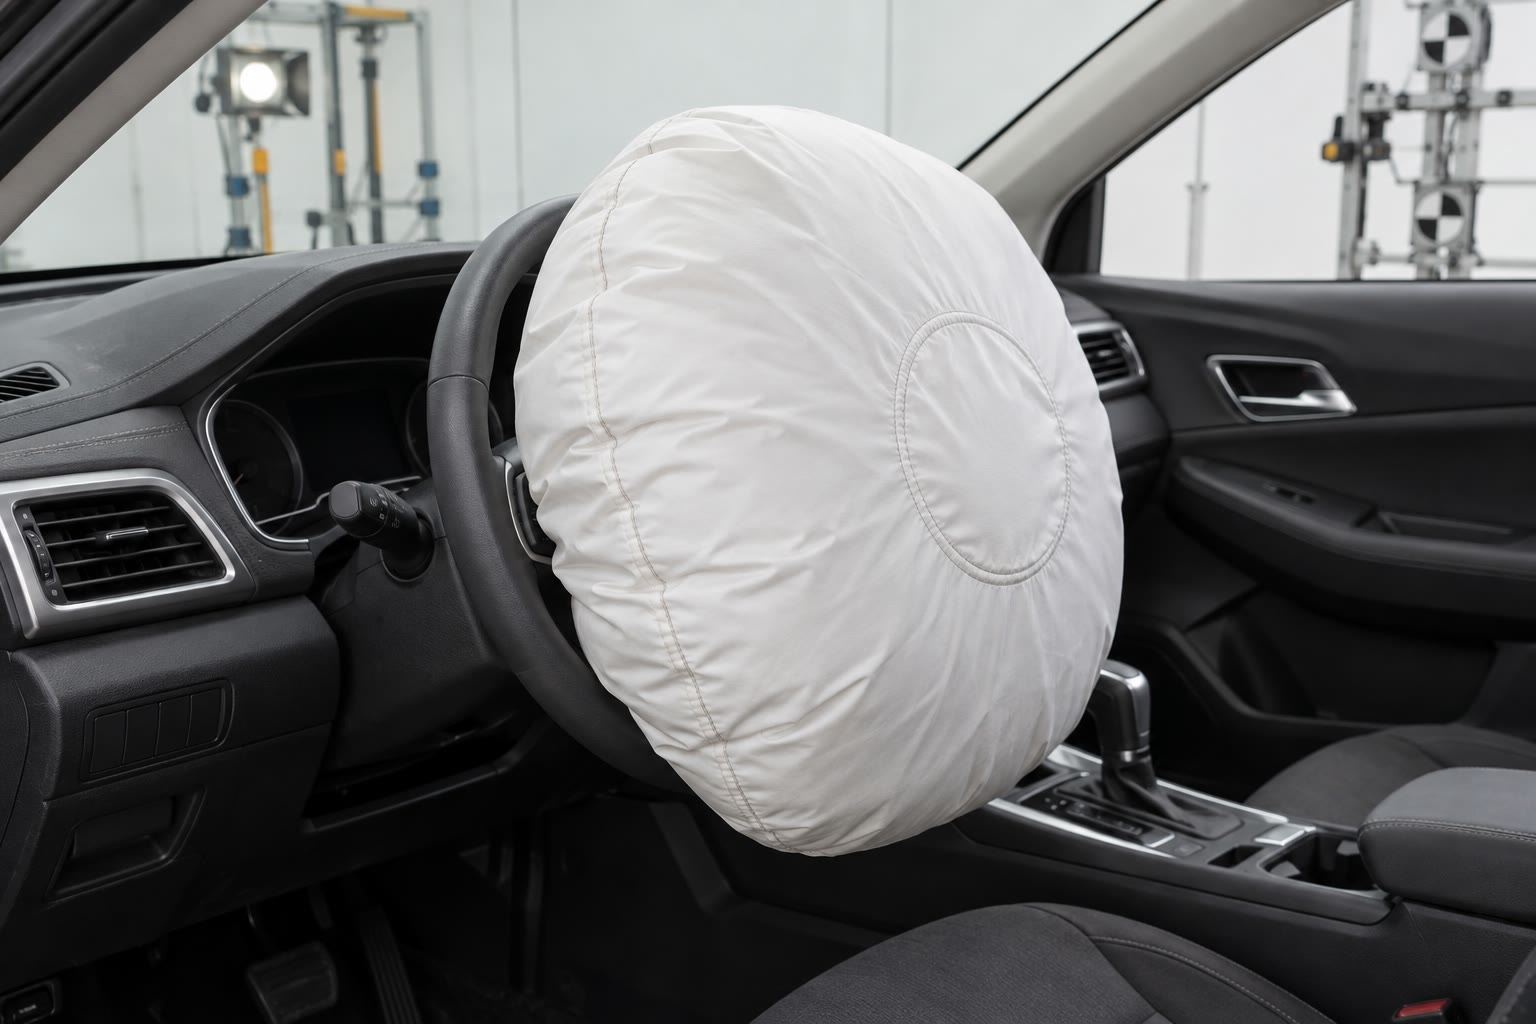
\includegraphics[width=0.5\linewidth]{images/book1/ai/g10-airbag.jpg}

{\small Kantong \omterm{def:g4:air-a-mixture-of-gases:air}{udara} terisi dalam sepersekian detik, dengan nitrogen
yang dihasilkan sebuah reaksi.}
\end{omfigure}

\section{Menggambarkan sebuah sistem kimia}

\begin{definition}[Sistem kimia, keadaan awal dan akhir]\label{def:g10:reaction-progress-table:system}
Yang disebut \emph{sistem kimia}\index{sistem kimia} adalah kumpulan
\omterm{def:g6:pure-substances-and-mixtures:species}{spesies kimia} yang ada di suatu tempat tertentu (sebuah labu, sebuah
bantalan, sebuah sel), masing-masing dengan \omterm{def:g10:the-mole:amount}{jumlah zat} dan wujudnya.
Sistem sebelum reaksi dimulai disebut
\emph{keadaan awal}\index{keadaan awal}; sistem setelah reaksi berhenti
disebut \emph{keadaan akhir}\index{keadaan akhir}.
\end{definition}


\begin{example}[Metana terbakar dalam bejana tertutup]\label{ex:g10:reaction-progress-table:methane}
Sebuah bejana tertutup berisi \qty{2.0}{mol} metana dan \qty{3.0}{mol}
gas oksigen; sebuah percikan api memicu \omterm{def:g4:what-a-fire-needs:burning}{pembakaran}
\ce{CH4 + 2O2 -> CO2 + 2H2O}. Pada \omterm{def:g10:reaction-progress-table:system}{keadaan awal} sistem itu memuat
\qty{2.0}{mol} \ce{CH4(g)}, \qty{3.0}{mol} \ce{O2(g)}, dan tidak ada
produk. Apa isi \omterm{def:g10:reaction-progress-table:system}{keadaan akhirnya}? Sisa bab ini menjawabnya.
\end{example}

\section{Kemajuan reaksi dan tabel kemajuan}

\begin{definition}[Kemajuan reaksi, tabel kemajuan]\label{def:g10:reaction-progress-table:extent}
Yang disebut \emph{kemajuan reaksi}\index{kemajuan reaksi} $x$, dalam
\omterm{def:g10:the-mole:amount}{mol}, menghitung berapa kali reaksi, seperti yang tertulis dalam
\omterm{def:g8:balanced-equations:equation}{persamaan setaranya}, telah berlangsung: ketika kemajuannya $x$, sebuah
spesies berkoefisien $\nu$ telah terpakai (\omterm{def:g7:chemical-reactions:reactant}{pereaksi}) atau terbentuk
(produk) sebanyak $\nu x$. Sebuah
\emph{tabel kemajuan}\index{tabel kemajuan} memberikan, di bawah
persamaan, \omterm{def:g10:the-mole:amount}{jumlah zat} setiap spesies pada \omterm{def:g10:reaction-progress-table:system}{keadaan awal}, pada kemajuan
$x$, dan pada \omterm{def:g10:reaction-progress-table:system}{keadaan akhir}.
\end{definition}

\begin{method}[Mengisi tabel kemajuan]\label{met:g10:reaction-progress-table:fill}
\begin{enumerate}
  \item Tuliskan \omterm{def:g8:balanced-equations:equation}{persamaan setara} di baris pertama.
  \item \omterm{def:g10:reaction-progress-table:system}{Keadaan awal} ($x = 0$): tuliskan jumlah awal setiap spesies di
        bawahnya.
  \item Keadaan antara (kemajuan $x$): setiap \omterm{def:g7:chemical-reactions:reactant}{pereaksi} berkoefisien
        $\nu$ menjadi $n_0 - \nu x$, setiap produk $n_0 + \nu x$.
  \item \omterm{def:g10:reaction-progress-table:system}{Keadaan akhir}: tentukan $x_{\max}$ (subbab berikutnya) lalu
        masukkan ke dalam ungkapan-ungkapan baris antara.
\end{enumerate}
\end{method}

\begin{omfigure}
\renewcommand{\arraystretch}{1.25}
\begin{tabular}{l|c|cccc}
\hline
persamaan & & \ce{CH4} & $+$ \ce{2O2} & $\longrightarrow$ \ce{CO2} & $+$ \ce{2H2O} \\
\hline
keadaan & kemajuan (\si{mol}) & \multicolumn{4}{c}{\omterm{def:g10:the-mole:amount}{jumlah zat} (\si{mol})} \\
\hline
awal & $0$ & $2.0$ & $3.0$ & $0$ & $0$ \\
antara & $x$ & $2.0 - x$ & $3.0 - 2x$ & $x$ & $2x$ \\
akhir & $x_{\max} = 1.5$ & $0.5$ & $0$ & $1.5$ & $3.0$ \\
\hline
\end{tabular}\par\medskip

{\small \omterm{def:g10:reaction-progress-table:extent}{Tabel kemajuan} \omterm{def:g4:what-a-fire-needs:burning}{pembakaran} metana pada contoh. Setiap kolom
mengikuti satu spesies; koefisien 2 pada \ce{O2} dan pada \ce{H2O}
menjadi $2x$.}
\end{omfigure}

\section{Pereaksi pembatas dan keadaan akhir}

\begin{definition}[Pereaksi pembatas, kemajuan maksimum, reaksi tuntas]\label{def:g10:reaction-progress-table:limiting}
Sebuah reaksi disebut \emph{reaksi tuntas}\index{reaksi tuntas} jika
reaksi itu baru berhenti ketika salah satu \omterm{def:g7:chemical-reactions:reactant}{pereaksinya} habis. \omterm{def:g7:chemical-reactions:reactant}{Pereaksi}
itu disebut \emph{pereaksi pembatas}\index{pereaksi pembatas}; \omterm{def:g7:chemical-reactions:reactant}{pereaksi}
lainnya berlebih. Kemajuan ketika \omterm{def:g7:chemical-reactions:reactant}{pereaksi} pembatas habis disebut
\emph{kemajuan maksimum}\index{kemajuan maksimum} $x_{\max}$; \omterm{def:g10:reaction-progress-table:system}{keadaan
akhir} sebuah reaksi tuntas adalah keadaan pada $x = x_{\max}$.
\end{definition}

\begin{method}[Menentukan pereaksi pembatas]\label{met:g10:reaction-progress-table:limiting}
\begin{enumerate}
  \item Untuk setiap \omterm{def:g7:chemical-reactions:reactant}{pereaksi}, selesaikan $n_0 - \nu x = 0$: \omterm{def:g7:chemical-reactions:reactant}{pereaksi} itu
        akan habis pada $x = n_0 / \nu$.
  \item Nilai terkecil di antaranya adalah $x_{\max}$; \omterm{def:g7:chemical-reactions:reactant}{pereaksi} yang
        memberikannya adalah \omterm{def:g10:reaction-progress-table:limiting}{pereaksi pembatas}.
  \item Masukkan $x_{\max}$ ke dalam baris antara untuk memperoleh
        \omterm{def:g10:reaction-progress-table:system}{keadaan akhir}; periksalah bahwa tidak ada \omterm{def:g10:the-mole:amount}{jumlah zat} yang negatif.
\end{enumerate}
\end{method}

\begin{example}[Kembali ke metana]\label{ex:g10:reaction-progress-table:methane-final}
Metana akan habis pada $x = 2.0/1 = \qty{2.0}{mol}$, gas oksigen pada
$x = 3.0/2 = \qty{1.5}{mol}$. Yang lebih kecil adalah \qty{1.5}{mol}:
oksigen adalah \omterm{def:g10:reaction-progress-table:limiting}{pereaksi pembatas} dan $x_{\max} = \qty{1.5}{mol}$.
\omterm{def:g10:reaction-progress-table:system}{Keadaan akhirnya} memuat \qty{0.5}{mol} metana yang tersisa, tanpa
oksigen, \qty{1.5}{mol} karbon dioksida, dan \qty{3.0}{mol} air.
\end{example}

\begin{omfigure}
\begin{tikzpicture}
\begin{axis}[width=0.78\linewidth, height=6.2cm, xmin=0, xmax=2.05,
    ymin=0, ymax=4.2, xlabel={kemajuan $x$ (\si{mol})},
    ylabel={jumlah zat (\si{mol})}, axis lines*=left, ymajorgrids,
    grid style={gray!20}, tick label style={font=\small},
    label style={font=\small}, xtick={0,0.5,1,1.5,2},
    legend style={font=\small, at={(1.02,0.5)}, anchor=west, draw=none},
    legend cell align=left]
  \addplot[very thick, omDef, domain=0:2] {2-x};
  \addplot[very thick, omThm, domain=0:1.5] {3-2*x};
  \addplot[very thick, omMeth, domain=0:2] {x};
  \addplot[very thick, omProp, domain=0:2] {2*x};
  \legend{\ce{CH4}, \ce{O2}, \ce{CO2}, \ce{H2O}}
  \addplot[dashed, black!60] coordinates {(1.5,0) (1.5,4.2)};
  \node[font=\small, anchor=south west] at (axis cs:1.5,3.55) {$x_{\max}$};
  \fill[black!8, opacity=0.6] (axis cs:1.5,0) rectangle (axis cs:2.05,4.2);
\end{axis}
\end{tikzpicture}

{\small \omterm{def:g10:the-mole:amount}{Jumlah zat} terhadap kemajuan pada contoh metana. Oksigen
(merah) mencapai nol lebih dulu, pada $x = \qty{1.5}{mol}$: reaksi
berhenti di situ, dan bagian yang diarsir tidak pernah tercapai.}
\end{omfigure}

\begin{remark}[Tidak semua reaksi tuntas]\label{rem:g10:reaction-progress-table:not-total}
Banyak reaksi berhenti sebelum ada \omterm{def:g7:chemical-reactions:reactant}{pereaksi} yang habis: reaksi itu
mencapai keadaan tempat \omterm{def:g7:chemical-reactions:reactant}{pereaksi} dan produk berada bersama-sama. \omterm{def:g10:reaction-progress-table:system}{Keadaan
akhirnya} bukan $x_{\max}$, dan sebuah bab berikutnya mempelajari cara
menentukannya. Dalam bab ini, setiap \omterm{def:g10:reaction-progress-table:limiting}{reaksi tuntas}.
\end{remark}

\section{Campuran stoikiometris}

\begin{definition}[Campuran stoikiometris]\label{def:g10:reaction-progress-table:stoichiometric}
Sebuah \omterm{def:g6:pure-substances-and-mixtures:mixture}{campuran} \omterm{def:g7:chemical-reactions:reactant}{pereaksi} disebut
\emph{campuran stoikiometris}\index{campuran stoikiometris} jika jumlah
awalnya sebanding dengan koefisien-koefisien \omterm{def:g8:balanced-equations:equation}{persamaan setaranya}.
\end{definition}

\begin{proposition}[Semua pereaksi habis bersama-sama]\label{prop:g10:reaction-progress-table:together}
Untuk reaksi $a\,\ce{A} + b\,\ce{B} \longrightarrow$ produk, \omterm{def:g6:pure-substances-and-mixtures:mixture}{campurannya} stoikiometris jika
dan hanya jika
\[
  \frac{n_0(\ce{A})}{a} = \frac{n_0(\ce{B})}{b},
\]
dan dalam hal itu, untuk \omterm{def:g10:reaction-progress-table:limiting}{reaksi tuntas}, kedua \omterm{def:g7:chemical-reactions:reactant}{pereaksi} habis terpakai
pada \omterm{def:g10:reaction-progress-table:system}{keadaan akhir}.
\end{proposition}

\begin{proof}
\ce{A} akan habis pada $x = n_0(\ce{A})/a$, \ce{B} pada $x = n_0(\ce{B})/b$.
Kedua nilai itu sama tepat ketika perbandingannya sama dengan
perbandingan dalam persamaan, dan dalam hal itu kemajuan $x_{\max}$
menghabiskan keduanya sekaligus.
\end{proof}

\begin{example}[Membakar metana dengan bersih]\label{ex:g10:reaction-progress-table:stoich}
Untuk \ce{CH4 + 2O2 -> CO2 + 2H2O}, \qty{2.0}{mol} metana memerlukan
\qty{4.0}{mol} gas oksigen: $2.0/1 = 4.0/2$. Dengan hanya
\qty{3.0}{mol} oksigen, \omterm{def:g6:pure-substances-and-mixtures:mixture}{campuran} pada contoh pertama kekurangan oksigen;
dalam nyala api yang sebenarnya, kekurangan itulah yang menghasilkan
karbon monoksida yang beracun (\cref{ch:g8:combustion-and-fuels}).
\end{example}

\section{Gas dan larutan dalam tabel}


\begin{method}[Jumlah zat untuk keadaan awal]\label{met:g10:reaction-progress-table:amounts}
Sebelum mengisi tabel, ubahlah setiap besaran yang diberikan menjadi
\omterm{def:g10:the-mole:amount}{jumlah zat}: $n = m/M$ untuk padatan atau cairan yang ditimbang;
$n = V/V_m$ untuk gas; $n = c \times V$ untuk spesies yang terlarut. Pada
akhirnya, ubahlah kembali \omterm{def:g10:the-mole:amount}{jumlah zat} pada \omterm{def:g10:reaction-progress-table:system}{keadaan akhir} menjadi apa pun
yang ditanyakan: massa, volume gas, atau konsentrasi.
\end{method}

\begin{example}[Magnesium dalam asam klorida]\label{ex:g10:reaction-progress-table:magnesium}
% ledger: aw:Mg
Asam klorida mengandung \omterm{def:g9:ions:ion}{ion} hidrogen \ce{H+}, yang menyerang magnesium:
\ce{Mg + 2H+ -> Mg^{2+} + H2}. Sepotong pita magnesium \qty{0.12}{g}
dijatuhkan ke dalam \qty{50.0}{mL} asam dengan
$c(\ce{H+}) = \qty{1.0}{mol/L}$. Jumlah awal:
$n_0(\ce{Mg}) = 0.12/24.3 = \qty{4.9e-3}{mol}$ dan
$n_0(\ce{H+}) = 1.0 \times 0.0500 = \qty{5.0e-2}{mol}$. Magnesium akan
habis pada $x = \qty{4.9e-3}{mol}$, \omterm{def:g9:ions:ion}{ion} hidrogen pada
$x = 0.050/2 = \qty{2.5e-2}{mol}$: magnesium adalah pembatas dan
$x_{\max} = \qty{4.9e-3}{mol}$. Reaksi itu menghasilkan \qty{4.9e-3}{mol}
gas hidrogen, yaitu $\num{4.9e-3} \times 24.1 = \qty{0.12}{L}$ pada
\qty{20}{\celsius}, dan menyisakan $0.050 - 2 \times 0.0049 =
\qty{0.040}{mol}$ \omterm{def:g9:ions:ion}{ion} hidrogen yang berlebih.
\end{example}

\begin{inthelab}[Balon pada labu]
Guru menuangkan \qty{50.0}{mL} asam klorida yang sama ke dalam masing-masing
dari enam labu Erlenmeyer, dan memasukkan ke dalam enam balon serbuk
magnesium dengan massa yang makin besar: 0.15, 0.30, 0.45, 0.60, 0.75,
dan \qty{0.90}{g}. Setiap balon dipasang menutupi leher labunya, lalu
diangkat sehingga serbuknya jatuh ke dalam asam. Sambil berdesis,
balon-balon itu menggembung. Ketika semuanya berhenti, balon-balon itu
makin besar dari labu pertama sampai labu keempat; balon keempat,
kelima, dan keenam sama besarnya, dan pada dua labu terakhir tersisa
sedikit serbuk kelabu di dasar labu.
\end{inthelab}

\begin{omfigure}
\begin{tikzpicture}[font=\small, scale=0.82]
  % H2 volume (L): 0.149 0.298 0.446 0.595 0.6025 0.6025; radius ~ V^(1/3)
  \foreach \i/\m/\v/\r/\left in {0/0.15/0.15/0.42/0, 1/0.30/0.30/0.53/0,
      2/0.45/0.45/0.61/0, 3/0.60/0.60/0.67/0, 4/0.75/0.60/0.67/1,
      5/0.90/0.60/0.67/1} {
    \begin{scope}[shift={(2.35*\i,0)}]
      \pic[transform shape] at (0,0) {erlenmeyer={0.25}{omWater}};
      \ifnum\left=1
        \fill[black!45] (-0.5,0.03) rectangle (0.5,0.12);
      \fi
      \fill[omProp!35, draw=omProp!80!black] (-0.3,2.6) -- (0.3,2.6)
        -- (0.12,2.82) -- (-0.12,2.82) -- cycle;
      \shade[ball color=omProp!40, draw=omProp!80!black]
        (0,{2.78+\r}) circle (\r);
      \node[align=center, anchor=north] at (0,-0.15)
        {\qty{\m}{g} Mg\\ \qty{\v}{L}};
    \end{scope}
  }
\end{tikzpicture}

{\small Enam labu dengan asam yang sama dan massa magnesium yang makin
besar, beserta volume gas hidrogen (pada \qty{20}{\celsius}) di dalam
setiap balon. Di atas sekitar \qty{0.61}{g}, asamlah yang menjadi
pembatas: balon-balon berhenti membesar dan magnesium tersisa
(kelabu).}
\end{omfigure}

\begin{remark}[Membaca bagian datar]\label{rem:g10:reaction-progress-table:plateau}
Pada labu-labu pertama magnesium adalah \omterm{def:g10:reaction-progress-table:limiting}{pereaksi pembatas}, dan
menggandakannya menggandakan gasnya. Mulai dari massa tertentu, \omterm{def:g9:ions:ion}{ion}
hidrogenlah yang habis lebih dulu: menambah magnesium tidak mengubah
apa pun selain serbuk yang tersisa. Perubahan itu terjadi tepat pada
\omterm{def:g10:reaction-progress-table:stoichiometric}{campuran stoikiometris}, $n_0(\ce{Mg}) = n_0(\ce{H+})/2 = \qty{0.025}{mol}$,
yaitu $0.025 \times 24.3 = \qty{0.61}{g}$ magnesium.
\end{remark}

\begin{safety}{\ghs[0.82cm]{GHS02}\ghs[0.82cm]{GHS05}\ghs[0.82cm]{GHS07}}
% ledger: ghs:Mg, ghs:HCl
Serbuk magnesium mudah menyala; asam klorida melukai kulit dan mata
serta uapnya mengiritasi saluran pernapasan; gas hidrogen \omterm{def:g4:what-a-fire-needs:burning}{terbakar} di
\omterm{def:g4:air-a-mixture-of-gases:air}{udara}. Ini demonstrasi oleh guru, dengan kacamata pelindung, jauh dari
nyala api apa pun.
\end{safety}

\section{Latihan}

\begin{exercise}[$\star$]\label{exo:g10:reaction-progress-table:1}
Isilah \omterm{def:g10:reaction-progress-table:extent}{tabel kemajuan} \ce{2H2 + O2 -> 2H2O} untuk \omterm{def:g6:pure-substances-and-mixtures:mixture}{campuran} awal
\qty{4.0}{mol} gas hidrogen dan \qty{3.0}{mol} gas oksigen, dengan
menganggap reaksinya tuntas. Tentukan $x_{\max}$, \omterm{def:g10:reaction-progress-table:limiting}{pereaksi pembatas}, dan
\omterm{def:g10:reaction-progress-table:system}{keadaan akhirnya}.
\end{exercise}

\begin{exercise}[$\star$]\label{exo:g10:reaction-progress-table:2}
Karbon \omterm{def:g4:what-a-fire-needs:burning}{terbakar} dalam gas oksigen: \ce{C + O2 -> CO2}. Mulai dari
\qty{3.0}{mol} karbon dan \qty{2.0}{mol} gas oksigen, tentukan
$x_{\max}$, \omterm{def:g10:reaction-progress-table:limiting}{pereaksi pembatas}, dan \omterm{def:g10:reaction-progress-table:system}{keadaan akhirnya}.
\end{exercise}

\begin{exercise}[$\star$]\label{exo:g10:reaction-progress-table:3}
Besi dan belerang bereaksi jika dipanaskan: \ce{Fe + S -> FeS}. Mulai
dari \qty{0.50}{mol} besi dan \qty{0.30}{mol} belerang, uraikan \omterm{def:g10:reaction-progress-table:system}{keadaan
akhirnya}.
\end{exercise}

\begin{exercise}[$\star$]\label{exo:g10:reaction-progress-table:4}
Anggaplah reaksi \ce{N2 + 3H2 -> 2NH3} tuntas. Mulai dari
\qty{1.0}{mol} gas nitrogen dan \qty{2.4}{mol} gas hidrogen, tentukan
$x_{\max}$ dan \omterm{def:g10:reaction-progress-table:system}{keadaan akhirnya}.
\end{exercise}

\begin{exercise}[$\star$]\label{exo:g10:reaction-progress-table:5}
Untuk \ce{2CO + O2 -> 2CO2}, manakah di antara \omterm{def:g6:pure-substances-and-mixtures:mixture}{campuran} berikut yang
stoikiometris? (a) \qty{2}{mol} \ce{CO} dan \qty{2}{mol} \ce{O2};
(b) \qty{4}{mol} \ce{CO} dan \qty{2}{mol} \ce{O2}; (c) \qty{1}{mol}
\ce{CO} dan \qty{2}{mol} \ce{O2}.
\end{exercise}

\begin{exercise}[$\star\star$]\label{exo:g10:reaction-progress-table:6}
Berapa massa gas oksigen yang diperlukan untuk membakar sempurna
\qty{32}{g} metana (\ce{CH4 + 2O2 -> CO2 + 2H2O})? Berapa massa air yang
terbentuk?
\end{exercise}

\begin{exercise}[$\star\star$]\label{exo:g10:reaction-progress-table:7}
Sebuah kompor kemah membakar \qty{1.0}{kg} propana:
\ce{C3H8 + 5O2 -> 3CO2 + 4H2O}. Berapa volume karbon dioksida, pada
\qty{20}{\celsius}, yang dilepaskannya?
\end{exercise}

\begin{exercise}[$\star\star$]\label{exo:g10:reaction-progress-table:8}
Dengan gambar \omterm{def:g10:the-mole:amount}{jumlah zat} terhadap kemajuan pada contoh metana, bacalah
\omterm{def:g10:the-mole:amount}{jumlah zat} keempat spesies pada $x = \qty{1.0}{mol}$. Mengapa garis gas
oksigen berhenti pada $x = \qty{1.5}{mol}$?
\end{exercise}

\begin{exercise}[$\star\star$]\label{exo:g10:reaction-progress-table:9}
Sebanyak \qty{1.30}{g} serbuk seng ditambahkan ke dalam \qty{100.0}{mL}
larutan tembaga sulfat biru \qty{0.10}{mol/L}. Reaksinya
\ce{Zn + Cu^{2+} -> Zn^{2+} + Cu}.
Tentukan \omterm{def:g10:reaction-progress-table:limiting}{pereaksi pembatas}, massa tembaga yang terbentuk, dan massa seng
yang tersisa. Apakah larutannya masih biru pada akhirnya?
\end{exercise}

\begin{exercise}[$\star\star$]\label{exo:g10:reaction-progress-table:10}
Sebanyak \qty{0.48}{g} magnesium ditambahkan ke dalam \qty{20.0}{mL} asam
klorida dengan $c(\ce{H+}) = \qty{1.0}{mol/L}$
(\ce{Mg + 2H+ -> Mg^{2+} + H2}). \omterm{def:g7:chemical-reactions:reactant}{Pereaksi} mana yang membatasi? Berapa
volume gas hidrogen yang ditampung pada \qty{20}{\celsius}?
\end{exercise}

\begin{exercise}[$\star\star$]\label{exo:g10:reaction-progress-table:11}
Pada latihan~3, berapa persen \omterm{def:g7:chemical-reactions:reactant}{pereaksi} yang berlebih melampaui jumlah
yang akan menghasilkan \omterm{def:g10:reaction-progress-table:stoichiometric}{campuran stoikiometris}?
\end{exercise}

\begin{exercise}[$\star\star\star$]\label{exo:g10:reaction-progress-table:12}
Seorang siswa menginginkan \qty{10.0}{g} \omterm{def:g10:reaction-progress-table:stoichiometric}{campuran stoikiometris} besi dan
belerang untuk \ce{Fe + S -> FeS}. Berapa massa besi dan massa belerang
yang harus ditimbang?
\end{exercise}

\begin{exercise}[$\star\star\star$]\label{exo:g10:reaction-progress-table:13}
Sebanyak \qty{10.0}{g} batu kapur \ce{CaCO3} dipanaskan dengan kuat dan
terurai seluruhnya: \ce{CaCO3 -> CaO + CO2}. Kapur tohor \ce{CaO} yang
diperoleh lalu dimasukkan ke dalam \qty{1.8}{g} air:
\ce{CaO + H2O -> Ca(OH)2}.
\begin{enumerate}
  \item Isilah tabel \omterm{def:g10:reaction-progress-table:extent}{kemajuan reaksi} pertama; berapa volume karbon
        dioksida yang dilepaskan pada \qty{20}{\celsius}?
  \item Isilah tabel reaksi kedua. \omterm{def:g7:chemical-reactions:reactant}{Pereaksi} mana yang membatasi? Berapa
        massa kapur padam \ce{Ca(OH)2} yang terbentuk?
\end{enumerate}
\end{exercise}

\begin{exercise}[$\star\star\star$]\label{exo:g10:reaction-progress-table:14}
Pada percobaan balon dalam kotak laboratorium, hitung volume gas
hidrogen di dalam setiap balon. Jelaskan mengapa balon berhenti membesar
setelah labu keempat, lalu gambarlah (dengan tangan) grafik volume gas
terhadap massa magnesium.
\end{exercise}

\begin{exercise}[$\star\star\star$]\label{exo:g10:reaction-progress-table:15}
Sebanyak \qty{4.6}{g} etanol \ce{C2H6O} \omterm{def:g4:what-a-fire-needs:burning}{terbakar} dalam bejana tertutup
yang berisi \qty{4.8}{L} gas oksigen pada \qty{20}{\celsius}:
\ce{C2H6O + 3O2 -> 2CO2 + 3H2O}. Tentukan \omterm{def:g10:reaction-progress-table:limiting}{pereaksi pembatas}, massa etanol
yang tersisa tidak \omterm{def:g4:what-a-fire-needs:burning}{terbakar}, dan volume karbon dioksida yang terbentuk.
\end{exercise}

\section{Soal: Kantong Udara}

\begin{problem}[{Soal akhir pekan --- berapa massa natrium azida yang harus
dimasukkan ke dalam roda kemudi untuk mengisi kantong udara 60 liter?}]
\label{pb:g10:reaction-progress-table:1}
% ledger: use:NaN3-airbag, ghs:NaN3, aw:Na, aw:N, aw:K, aw:O
Pada rancangan kantong \omterm{def:g4:air-a-mixture-of-gases:air}{udara} yang klasik, sebuah percikan listrik memicu
penguraian padatan natrium azida:
\[
  \ce{2NaN3 -> 2Na + 3N2} .
\]
\omterm{def:g9:periodic-table-first-look:metal}{Logam} natrium yang terbentuk berbahaya: \omterm{def:g9:periodic-table-first-look:metal}{logam} itu bereaksi hebat dengan
air, dan dengan kelembapan kulit dan mata. Karena itu muatannya juga
mengandung kalium nitrat, yang mengubah natrium menjadi oksida-oksida
yang tidak berbahaya dan menghasilkan sedikit nitrogen tambahan:
\[
  \ce{10Na + 2KNO3 -> K2O + 5Na2O + N2} .
\]
Kedua reaksi itu tuntas. Kantong \omterm{def:g4:air-a-mixture-of-gases:air}{udara} itu harus diisi dengan
\qty{60}{L} nitrogen; anggaplah gas itu pada \qty{20}{\celsius}, dengan
$V_m = \qty{24.1}{L/mol}$.

\medskip
\noindent\textbf{Bagian I --- Reaksi-reaksinya.}
\begin{enumerate}
  \item Periksalah bahwa persamaan pertama setara, unsur demi unsur.
  \item Periksalah bahwa persamaan kedua setara.
  \item Bab mana sebelumnya yang menunjukkan bahwa natrium bereaksi hebat
        dengan air? Mengapa tidak boleh ada natrium yang tersisa setelah
        tabrakan?
  \item Hitung \omterm{def:g10:the-mole:molar-mass}{massa molar} natrium azida \ce{NaN3} dan kalium nitrat
        \ce{KNO3}.
\end{enumerate}

\medskip
\noindent\textbf{Bagian II --- Penguraian.}
\begin{enumerate}[resume]
  \item Isilah tabel \omterm{def:g10:reaction-progress-table:extent}{kemajuan reaksi} pertama untuk jumlah awal
        \qty{1.00}{mol} natrium azida.
  \item Tentukan $x_{\max}$. Mana \omterm{def:g10:reaction-progress-table:limiting}{pereaksi pembatasnya}?
  \item Berikan \omterm{def:g10:the-mole:amount}{jumlah zat} natrium dan nitrogen pada \omterm{def:g10:reaction-progress-table:system}{keadaan akhir}.
  \item Berapa volume nitrogen yang dihasilkan \qty{1.00}{mol} natrium
        azida pada \qty{20}{\celsius}?
\end{enumerate}

\medskip
\noindent\textbf{Bagian III --- Menghilangkan natrium.}
\begin{enumerate}[resume]
  \item Isilah tabel \omterm{def:g10:reaction-progress-table:extent}{kemajuan reaksi} kedua, mulai dari natrium yang
        diperoleh pada soal 7 dan jumlah $n$ kalium nitrat.
  \item Berapa \omterm{def:g10:the-mole:amount}{jumlah zat}, dan berapa massa, kalium nitrat yang membentuk
        \omterm{def:g10:reaction-progress-table:stoichiometric}{campuran stoikiometris} dengan natrium ini?
  \item Berikan \omterm{def:g10:reaction-progress-table:system}{keadaan akhir} reaksi kedua untuk \omterm{def:g6:pure-substances-and-mixtures:mixture}{campuran} ini.
  \item Jika hanya \qty{0.150}{mol} kalium nitrat yang dimasukkan,
        \omterm{def:g7:chemical-reactions:reactant}{pereaksi} mana yang akan menjadi pembatas, dan apa yang akan
        tersisa? Mengapa hal itu berbahaya?
\end{enumerate}

\medskip
\noindent\textbf{Bagian IV --- Kantong 60 liter.}
\begin{enumerate}[resume]
  \item Dari soal 7 dan 11, berapa \omterm{def:g10:the-mole:amount}{jumlah zat} nitrogen yang dihasilkan
        seluruh muatan itu per \omterm{def:g10:the-mole:amount}{mol} natrium azida?
  \item Berapa \omterm{def:g10:the-mole:amount}{jumlah zat} nitrogen yang mengisi kantong itu?
  \item Simpulkan \omterm{def:g10:the-mole:amount}{jumlah zat} natrium azida yang diperlukan.
  \item Hitung massanya.
  \item Hitung massa kalium nitrat yang harus ditambahkan.
  \item Tanpa reaksi kedua, berapa massa natrium azida yang akan
        diperlukan? Berapa banyak yang dihemat oleh reaksi kedua?
  \item Natrium azida berakibat fatal jika tertelan. Mengapa penting
        bahwa reaksi pertama tuntas, dan bagaimana \omterm{def:g10:reaction-progress-table:extent}{tabel kemajuan}
        menunjukkan bahwa tidak ada yang tersisa?
  \item Nyatakan jawaban akhirnya: berapa massa natrium azida yang
        mengisi kantong \omterm{def:g4:air-a-mixture-of-gases:air}{udara} \qty{60}{L}?
\end{enumerate}
\end{problem}
